\documentclass[11pt,a4paper]{article}
\usepackage{fontspec}
\setmainfont{Latin Modern Roman}
\setsansfont{Latin Modern Sans}
\usepackage[english]{babel}
\usepackage[margin=2.3cm]{geometry}
\usepackage{amsmath,amssymb,graphicx,booktabs,array,float,xcolor}
\usepackage{hyperref}
\hypersetup{colorlinks=true,linkcolor=black,urlcolor=blue!45!black,citecolor=blue!45!black}
\graphicspath{{figures/}}
\setlength{\parindent}{0pt}
\setlength{\parskip}{0.42em}
\renewcommand{\arraystretch}{1.14}
\begin{document}
\begin{center}
{\small FPT UNIVERSITY, HO CHI MINH CITY CAMPUS \quad | \quad IMP302 MINI PROJECT\par}
\vspace{0.55em}
{\LARGE\bfseries Gaussian Image Denoising with Noise-Conditional, Data-Fitted Filter Fusion\par}
\vspace{0.55em}
{\normalsize Huỳnh Quốc Việt (SE194225) \qquad Lê Nguyễn Gia Hưng (SE194127)\par}
{\small Instructor: NguyenLP9 \quad | \quad 31 October 2026\par}
\vspace{0.45em}\hrule
\end{center}

\begin{abstract}
This study investigates Gaussian denoising of grayscale natural images from the Berkeley Segmentation Dataset (BSDS300). Gaussian smoothing, bilateral filtering, and Non-Local Means (NLM) provide interpretable baselines. The main method fits a nonnegative, sum-to-one combination of their outputs separately for three noise levels; a small residual multilayer perceptron (MLP) tests whether pixelwise nonlinear correction adds value. Sixty images fit weights, 12 select NLM and MLP settings, 20 pilot images informed development, and a separate 20-image set supplies the final results. At noise standard deviations 15, 25, and 50, fusion achieves mean PSNRs of 29.18, 26.72, and 23.61 dB. Its paired gains over the strongest individual PSNR baseline, bilateral filtering, are 0.37, 0.37, and 0.49 dB; the residual MLP does not improve on fusion. We provide image-level scores, paired bootstrap intervals, executable EDA notebooks, a local web demonstration, and reproducibility records. Conclusions are limited to the fixed grayscale subset and synthetic noise protocol.
\end{abstract}
\textbf{Keywords:} image denoising; Gaussian noise; filter fusion; Non-Local Means; residual learning; BSDS300.

\section{Introduction}
Noise reduction is a compact way to connect IMP302 topics: spatial linear and nonlinear filtering (Chapter 2), degradation and restoration (Chapter 3), image quality assessment (Chapter 8), and feature extraction and neural models (Chapters 10--12). The course handouts are mapped in \texttt{docs/course-map.md}. Our question is whether a filter mixture, fitted on training images for each noise level, generalizes better than any of its individual filters on held-out images. A residual MLP is a deliberately small nonlinear comparison, rather than a presumed superior method.

The contribution is an auditable course-scale comparison: fixed image-level splits, recorded data and seeds, identical noisy inputs for every method, validation-only setting selection, paired final-test analysis, and a working demo. This is an application and measurement study, not a claim to have invented filter fusion or residual denoising.

\section{Related work}
Gaussian smoothing averages nearby values and is fast, but can blur edges. The bilateral filter also weights intensity similarity to better preserve boundaries \cite{tomasi1998}. NLM exploits repeated patches beyond the immediate neighborhood \cite{buades2005}. Residual-learning denoisers such as DnCNN establish that learned corrections are a mature direction \cite{zhang2017}; combining nonlocal algorithms with neural correction has also been studied \cite{guo2021}. Our MLP is much smaller and pixelwise, and our main method is a constrained mixture of three classical outputs. Its practical novelty within this mini project is that the weights are learned rather than set equally, and they vary with the known synthetic noise level. We test that design empirically rather than claiming field-level novelty.

\section{Materials and methods}
\subsection{Data, preprocessing, and exploratory audit}
Images come from the official BSDS300 image archive \cite{berkeley,martin2001}. Although BSDS300 was released for segmentation research, we use only its photographs, not segmentation labels. The archive URL and SHA-256 are saved in \path{data/manifest.json}. The verified digest is
\begin{center}\small\texttt{7f855a00491a3f1ca2609b3c96651b88b2}\\\texttt{65fe59b70a7b007cc7a2850a22b386}\end{center}
Intended use is noncommercial education and research. Each original JPEG is decoded to 8-bit grayscale and resized so its longer side is at most 256 pixels. The decoded JPEG is the reference, not an ideal camera-sensor ground truth.

The original BSDS300 training split supplies 60 training and 12 validation images. The first 20 sorted IDs of the original test split formed a development pilot. After observing that the MLP did not improve consistently, the fusion design was added; the \emph{next} 20 original-test IDs became the final held-out set. Therefore the pilot is not included in final tables, and the 20-image final set is not the full BSDS300 test split. All IDs are fixed in the manifest.

Notebook~\texttt{01\_dataset\_eda.ipynb} verified all 112 processed files, unique split IDs, and no exact cross-split duplicates. A dHash screening threshold of Hamming distance at most 4 produced zero cross-split candidates; this is a limited duplicate screen, not a proof of semantic independence. Train images span mean brightness 45.58--167.75 gray levels and have dimensions from 171 to 256 pixels per side. Figure~\ref{fig:eda} shows train-only property distributions. These audit and training-image observations did not use held-out test pixels to choose features or parameters.

\begin{figure}[ht]
\centering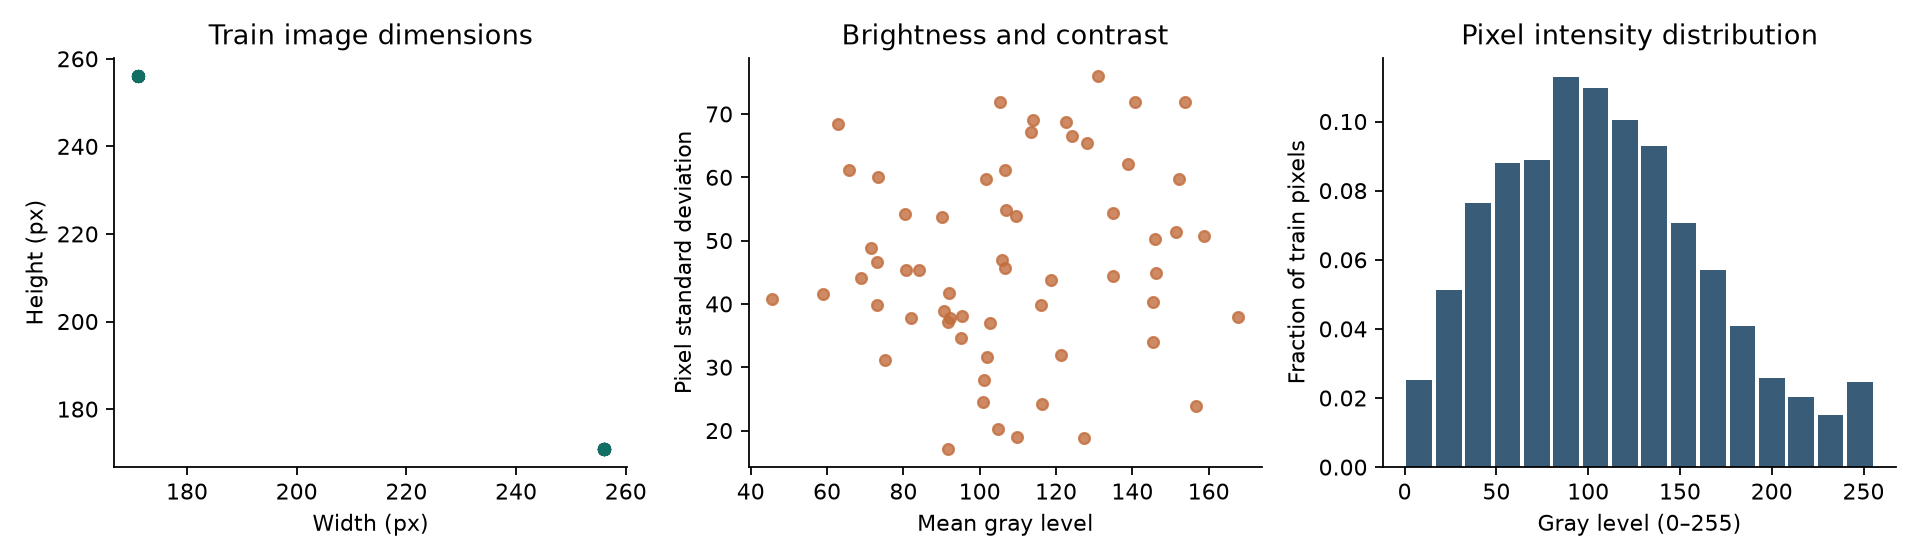
\includegraphics[width=0.92\textwidth]{eda_train_properties.png}
\caption{Train-only image dimensions, mean brightness versus pixel standard deviation, and the 16-bin grayscale intensity distribution. Generated by Notebook 01.}
\label{fig:eda}
\end{figure}

For clean reference $x$ and independent Gaussian noise $n\sim\mathcal N(0,\sigma^2)$, the shared noisy input is $y=\operatorname{clip}_{[0,255]}(x+n)$ after 8-bit conversion, with $\sigma\in\{15,25,50\}$. Seed 302 is derived per image ID and noise level. Clipping makes measured differences near black or white depart from an unbounded Gaussian; the train-only noise example in Notebook 01 records this effect.

\subsection{Classical filters and validation selection}
For a noisy image $y$, let $g$, $b$, and $m$ be Gaussian, bilateral, and NLM outputs. OpenCV parameters are fixed as follows: Gaussian kernel $5\times5$ with spatial standard deviation 1.1; bilateral diameter 7, color standard deviation $2.5\sigma$, spatial standard deviation 3; NLM patch size $7\times7$ and search size $21\times21$. NLM strength $h$ is selected by mean PSNR on the 12 validation images, independently for each noise level; the selected values are 16, 24, and 40. The full search grid and scores are in \texttt{results/nlm\_tuning.csv}. The Gaussian and bilateral settings are fixed baselines and were not exhaustively optimized.

\subsection{Noise-conditional fusion}
Our main estimate combines the three filter outputs at each pixel $p$:
\begin{equation}
\hat x^{\mathrm{fusion}}_p=\operatorname{clip}_{[0,255]}\!\left(w_{g,\sigma}g_p+w_{b,\sigma}b_p+w_{m,\sigma}m_p\right),
\qquad w_{k,\sigma}\geq 0,\quad \sum_k w_{k,\sigma}=1.
\end{equation}
For each $\sigma$, we enumerate weights on a simplex grid in increments of 0.05 and minimize training mean squared error. Each of 60 train images contributes 700 randomly sampled pixels per noise level, giving 126,000 training samples in total. The design has two free weights per level and is interpretable. Learned weights are stored in \texttt{models/fusion.json}; Table~\ref{tab:weights} reports them.

\subsection{Residual MLP and feature analysis}
The comparison MLP predicts a correction to NLM. Its ten inputs per pixel are $y/255$, $g/255$, $b/255$, $m/255$, $(y-m)/50$, $(b-m)/50$, $\sigma/50$, local mean$/255$, local standard deviation$/50$, and Sobel gradient magnitude$/400$. The local statistics use a $5\times5$ Gaussian neighborhood. These quantities expose brightness, filter disagreement, noise level, texture, and edges. Figure~\ref{fig:features} visualizes all channels on a train image; it shows available information, not feature importance.

\begin{figure}[ht]
\centering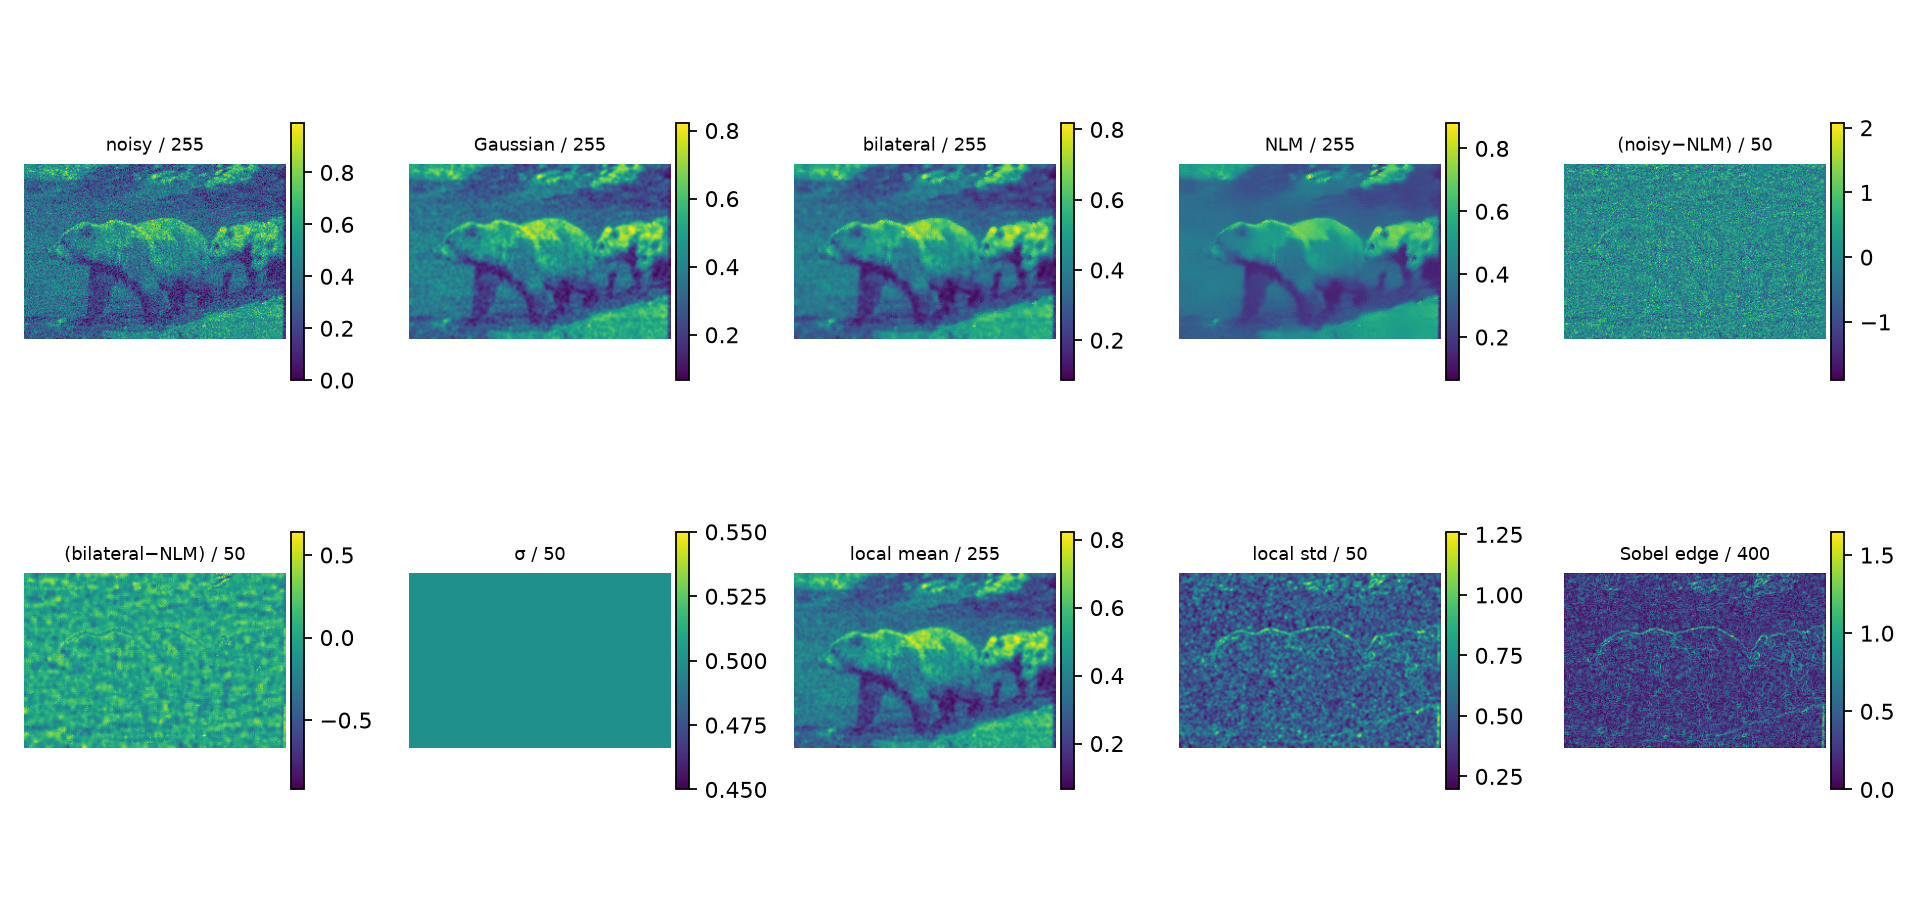
\includegraphics[width=0.92\textwidth]{eda_feature_maps.png}
\caption{The ten per-pixel MLP feature maps for one training image at $\sigma=25$, produced by Notebook 02. Colors are scaled separately per map; they are not comparable physical units.}
\label{fig:features}
\end{figure}

After featurewise normalization using train-only means and standard deviations, the network is
\begin{equation}
\hat r_p=W_2\operatorname{ReLU}(W_1\tilde\phi_p+b_1)+b_2,
\qquad \hat x^{\mathrm{MLP}}_p=\operatorname{clip}_{[0,255]}(m_p+255\hat r_p).
\end{equation}
The target is $(x_p-m_p)/255$. NumPy Adam trains the model from scratch for 12 epochs, batch size 2048, learning rate 0.001. Validation PSNR chooses among 16 units without texture, 16 with texture, and 32 with texture; 32 with texture wins (Table~\ref{tab:ablation}). There is no pretrained checkpoint. In this report, ``tuning'' means validation-based parameter and architecture selection, not fine-tuning a pretrained network. The final test was never used for either choice.

\subsection{Evaluation protocol}
For 8-bit images, $\mathrm{PSNR}=10\log_{10}(255^2/\mathrm{MSE})$. SSIM uses an $11\times11$ Gaussian window with standard deviation 1.5, $C_1=(0.01\cdot255)^2$, and $C_2=(0.03\cdot255)^2$ \cite{wang2004}; a five-pixel border is excluded from its mean. We average each metric \emph{per image} and then across the 20 final-test IDs at each noise level. For paired PSNR differences on the same images, 5,000 seeded image-level bootstrap resamples yield percentile 95\% intervals. Those intervals describe this fixed-image, fixed-noise protocol, not all natural photographs.

\section{Results}
% Generated from results/*.csv; measured values are not edited by hand.
\begin{table}[ht]
\centering\small
\caption{Mean PSNR (dB) / SSIM on 20 held-out test images per noise level.}
\label{tab:main}
\begin{tabular}{lccc}
\toprule
Method & $\sigma=15$ & $\sigma=25$ & $\sigma=50$ \\
\midrule
Noisy input & 24.77 / 0.619 & 20.49 / 0.440 & 14.94 / 0.226 \\
Gaussian & 26.58 / 0.762 & 25.66 / 0.702 & 23.00 / 0.548 \\
Bilateral & 28.81 / 0.819 & 26.35 / 0.723 & 23.12 / 0.554 \\
NLM & 28.63 / 0.812 & 26.19 / 0.722 & 23.00 / 0.567 \\
Learned fusion & 29.18 / 0.829 & 26.72 / 0.746 & 23.61 / 0.595 \\
Residual MLP & 28.24 / 0.797 & 26.08 / 0.690 & 23.21 / 0.513 \\
\bottomrule
\end{tabular}
\end{table}

\begin{table}[ht]
\centering\small
\caption{Paired fusion gains; 95\% image bootstrap intervals. MSE reduction is the geometric-mean equivalent of mean $\Delta$PSNR.}
\label{tab:paired}
\begin{tabular}{c l c c c c}
\toprule
$\sigma$ & Baseline & $\Delta$ dB & 95\% CI & Wins & MSE reduction \\
\midrule
15 & NLM & +0.55 & [+0.44, +0.65] & 19/20 & 11.9\% \\
25 & NLM & +0.54 & [+0.40, +0.68] & 18/20 & 11.6\% \\
50 & NLM & +0.61 & [+0.42, +0.77] & 18/20 & 13.1\% \\
15 & Bilateral & +0.37 & [+0.23, +0.52] & 16/20 & 8.2\% \\
25 & Bilateral & +0.37 & [+0.23, +0.53] & 17/20 & 8.2\% \\
50 & Bilateral & +0.49 & [+0.35, +0.67] & 20/20 & 10.7\% \\
\bottomrule
\end{tabular}
\end{table}

\begin{table}[ht]
\centering\small
\caption{Fusion weights fitted on training images; each row sums to one.}
\label{tab:weights}
\begin{tabular}{cccc}
\toprule
$\sigma$ & Gaussian & Bilateral & NLM \\
\midrule
15 & 0.10 & 0.40 & 0.50 \\
25 & 0.25 & 0.25 & 0.50 \\
50 & 0.45 & 0.05 & 0.50 \\
\bottomrule
\end{tabular}
\end{table}

\begin{table}[ht]
\centering\small
\caption{MLP ablation and configuration selection on validation images.}
\label{tab:ablation}
\begin{tabular}{ccc}
\toprule
Hidden units & Texture features & Validation PSNR (dB) \\
\midrule
16 & No & 23.71 \\
16 & Yes & 25.80 \\
32 & Yes & 26.43 \\
\bottomrule
\end{tabular}
\end{table}


Fusion reaches mean PSNRs of 29.18, 26.72, and 23.61 dB at $\sigma=15,25,50$ and SSIMs of 0.829, 0.746, and 0.595 (Table~\ref{tab:main}). Bilateral is the highest-PSNR individual filter at each level. Paired fusion gains over bilateral are 0.37, 0.37, and 0.49 dB; their bootstrap intervals exclude zero (Table~\ref{tab:paired}). Converting mean $\Delta$PSNR to a geometric-mean equivalent gives 8.2\%, 8.2\%, and 10.7\% lower MSE. Those percentages are \emph{not} percentage changes in PSNR. Fusion weights (Table~\ref{tab:weights}) assign more weight to Gaussian at higher noise in this fitted sample; this pattern is descriptive, not a universal law.

The residual MLP scores below fusion for both PSNR and SSIM at all three levels (Table~\ref{tab:main}). Thus the added pixelwise nonlinearity did not help under this data and training budget. Figure~\ref{fig:psnr} shows the aggregate PSNR trends, while Figure~\ref{fig:comparison} gives one visual example. A single example is illustrative and cannot substitute for paired scores across images.

\begin{figure}[ht]
\centering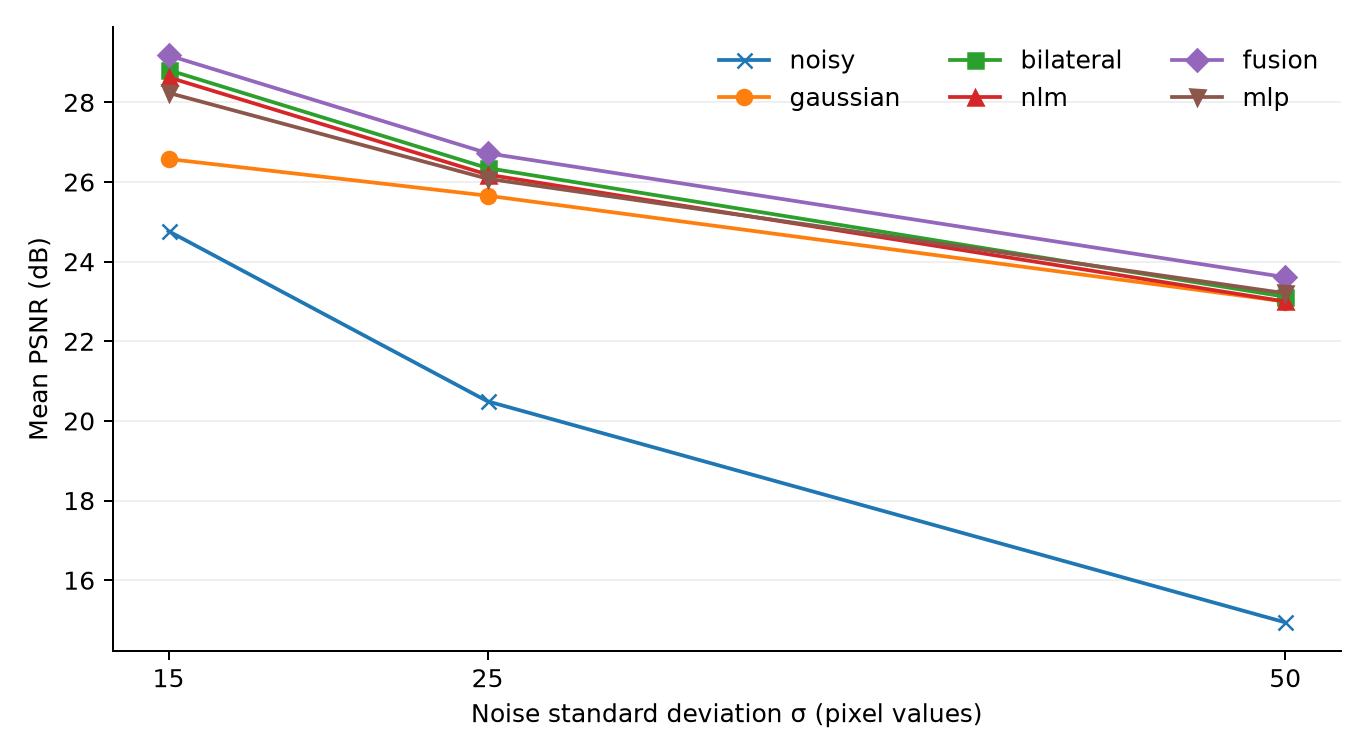
\includegraphics[width=0.76\textwidth]{psnr_by_noise.png}
\caption{Mean final-test PSNR by noise level, calculated from 20 held-out images per level. Higher dB means lower mean squared error.}
\label{fig:psnr}
\end{figure}

\begin{figure}[H]
\centering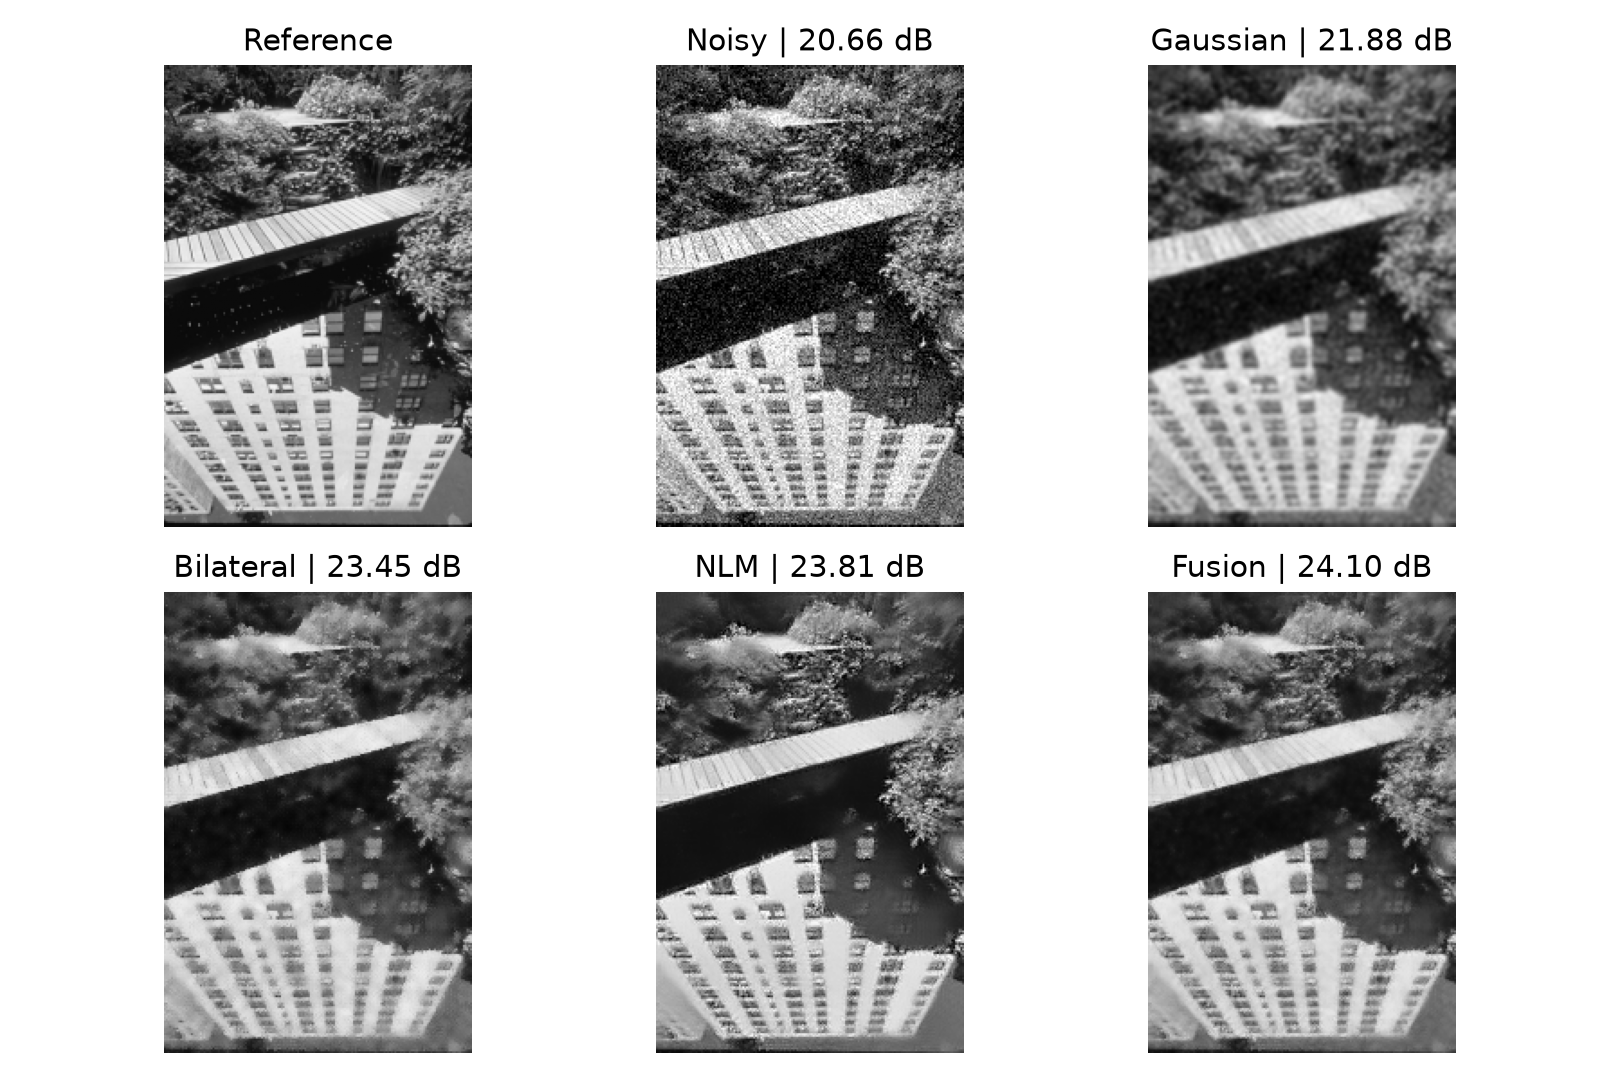
\includegraphics[width=0.86\textwidth]{comparison.png}
\caption{One held-out test image at $\sigma=25$, with identical noisy input and reference for each method. Aggregate results are in Table~\ref{tab:main}.}
\label{fig:comparison}
\end{figure}

\section{Discussion and limitations}
The constrained mixture is a useful update to equal-weight fusion in this study because train-fitted weights adapt to the specified noise level and can be inspected. The measured gain is modest, and related denoising and neural-correction methods predate this project \cite{buades2005,zhang2017,guo2021}. The MLP result cautions against assuming that more features and nonlinear capacity necessarily improve image restoration. Its pixelwise head cannot directly combine a broad spatial neighborhood, whereas NLM already encodes nonlocal patch evidence.

Interpretation has several limits. The final set contains only 20 fixed images from one source, selected after a separate pilot was seen during development. The noise is independent and synthetic, and the reference is a compressed JPEG converted to grayscale. Gaussian and bilateral hyperparameters were not exhaustively searched, so stronger optimized baselines may narrow the gain. PSNR and SSIM miss some perceptual qualities, and dHash cannot rule out every near duplicate. These results do not establish performance on color images, real camera noise, or another dataset. Any new design prompted by the final test would require a fresh untouched test set for a new confirmatory claim.

\section{Reproducibility and conclusion}
The dataset manifest records the source, archive hash, and split IDs. Run metadata records the seed and Python/NumPy/OpenCV versions. The experiment script writes image scores, validation searches, weights, bootstrap intervals, and figures. Notebook 01 saves the EDA summary; Notebook 02 documents features and model selection. A report script generates all tables from saved CSV/JSON, never from hand-transcribed values. The local web demo runs the same saved model and filters. The main finding is a measured improvement from simple train-fitted fusion over individual filters in the stated protocol, accompanied by a transparent negative MLP result.

\begin{thebibliography}{9}
\small\setlength{\itemsep}{0pt}\setlength{\parsep}{0pt}
\bibitem{berkeley} UC Berkeley, \emph{The Berkeley Segmentation Dataset and Benchmark}, \url{https://www2.eecs.berkeley.edu/Research/Projects/CS/vision/bsds/}.
\bibitem{martin2001} D. Martin, C. Fowlkes, D. Tal, J. Malik, ``A Database of Human Segmented Natural Images and its Application to Evaluating Segmentation Algorithms and Measuring Ecological Statistics,'' \emph{ICCV}, 2001, pp. 416--423. \url{https://www2.eecs.berkeley.edu/Research/Projects/CS/vision/grouping/papers/mftm-iccv01.pdf}.
\bibitem{tomasi1998} C. Tomasi and R. Manduchi, ``Bilateral Filtering for Gray and Color Images,'' \emph{ICCV}, 1998. \url{https://doi.org/10.1109/ICCV.1998.710815}.
\bibitem{buades2005} A. Buades, B. Coll, and J.-M. Morel, ``A Non-Local Algorithm for Image Denoising,'' \emph{CVPR}, 2005. \url{https://doi.org/10.1109/CVPR.2005.38}.
\bibitem{wang2004} Z. Wang, A. C. Bovik, H. R. Sheikh, and E. P. Simoncelli, ``Image Quality Assessment: From Error Visibility to Structural Similarity,'' \emph{IEEE Transactions on Image Processing}, 13(4), 2004, pp. 600--612. \url{https://www.cns.nyu.edu/pub/lcv/wang03-reprint.pdf}.
\bibitem{zhang2017} K. Zhang et al., ``Beyond a Gaussian Denoiser: Residual Learning of Deep CNN for Image Denoising,'' \emph{IEEE Transactions on Image Processing}, 26(7), 2017. \url{https://arxiv.org/abs/1608.03981}.
\bibitem{guo2021} Y. Guo, A. Davy, G. Facciolo, J.-M. Morel, and Q. Jin, ``Fast, Nonlocal and Neural: A Lightweight High Quality Solution to Image Denoising,'' \emph{IEEE Signal Processing Letters}, 28, 2021, pp. 1515--1519. \url{https://arxiv.org/abs/2403.03488}.
\end{thebibliography}
\end{document}
